\chapter{Estado del arte}

La motivación de este proyecto surge precisamente por el estado actual de los editores de imágenes. 
La mayoría de usuarios, edita el contenido que sube online desde una aplicación local instalada en 
su ordenador (Microsoft Paint, Photoshop), o en el caso de los que emplean aplicaciones en la nube, 
descargan sus imágenes para luego resubirlas a sus redes.
Concretamente los memes suelen ser ediciones especialmente simples, donde se añade un texto, 
se superponen varias imágenes o se dibuja algo encima de una imagen base.
\\\\
Este proyecto tiene como objetivo tratar este problema y evitar en la medida de lo posible el uso 
del almacenamiento local de imágenes, tanto para crear, como para subir el contenido ya editado. 
\\\\
Además, existen editores especialmente dedicados a los memes que te aportan varias plantillas
base, pero tienen muchas desventajas, en primer lugar los mas populares son toscos y desfasados,
con interfaces poco interactivas y sin mucha personalización, la edición es lenta y están faltos
de herramientas esenciales en el diseño de memes actual. 
\\\\
Desde hace años los memes han 
evolucionado y ya no se basan en una simple imagen con un texto, suelen ser una superposición
de varias imágenes, con elementos resaltados, muchos textos pequeños con diferentes estilos
y filtros o efectos.

\begin{figure}[!h]
\centering
    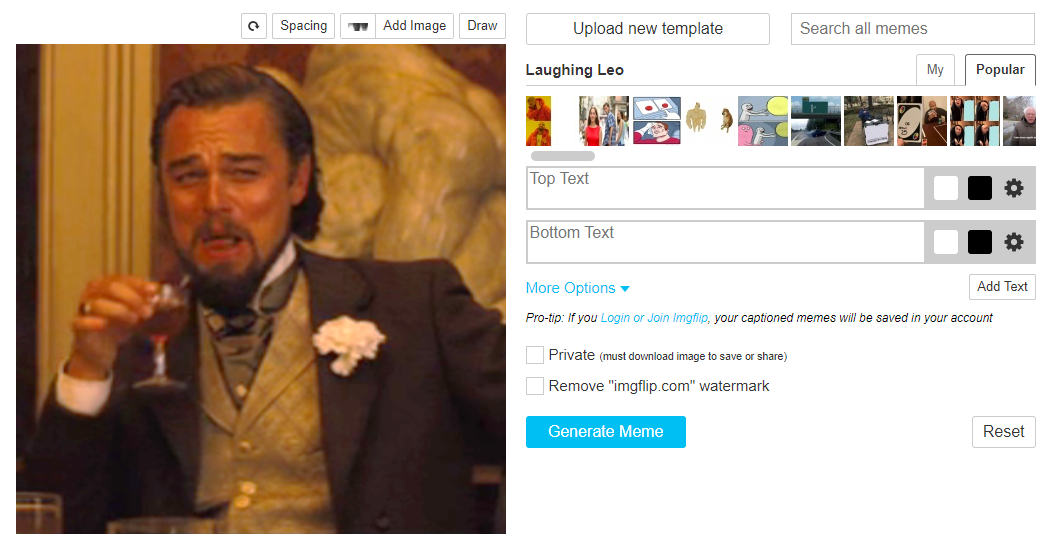
\includegraphics[scale=0.4]{img/imgflip.png}
\caption{imgflip, editor de memes popular.}
\end{figure}